\documentclass[main.tex]{subfiles}


\begin{document}

\section{Supplementary Figures}
\label{suppfigs}


\begin{suppfigure}[H]
	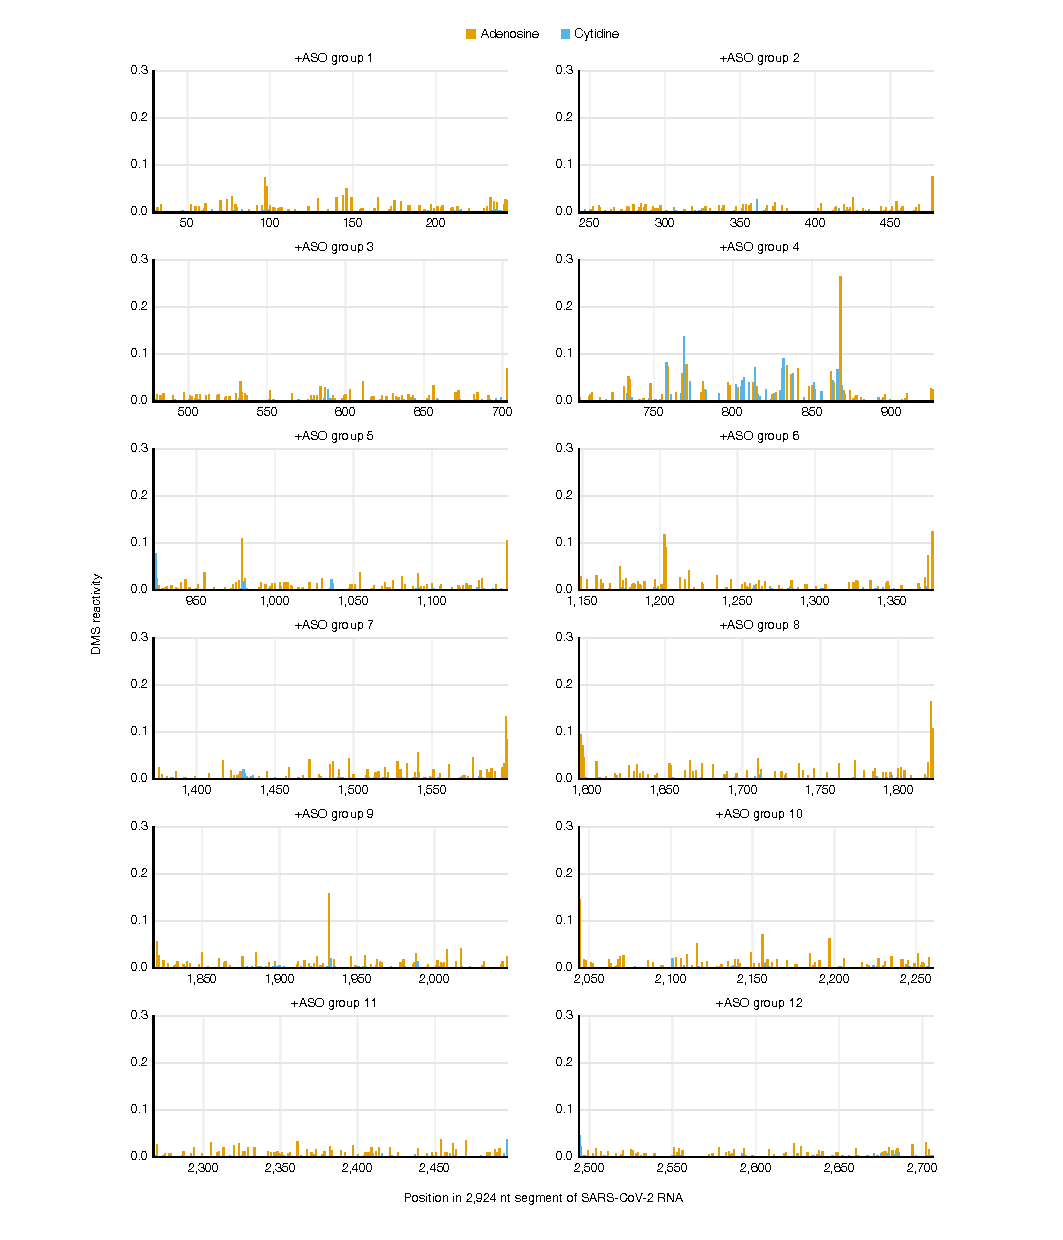
\includegraphics[width=\textwidth]{../SupplementaryFigures/sars2-tile-target.pdf}
	\caption{\textbf{Mutational profile of each ASO target section upon adding the corresponding group of ASOs to the 2,924 nt segment of SARS-CoV-2 genomic RNA.} Positions are colored based on the RNA sequence.}
	\label{sars2-tile-target}
\end{suppfigure}


\begin{suppfigure}[H]
	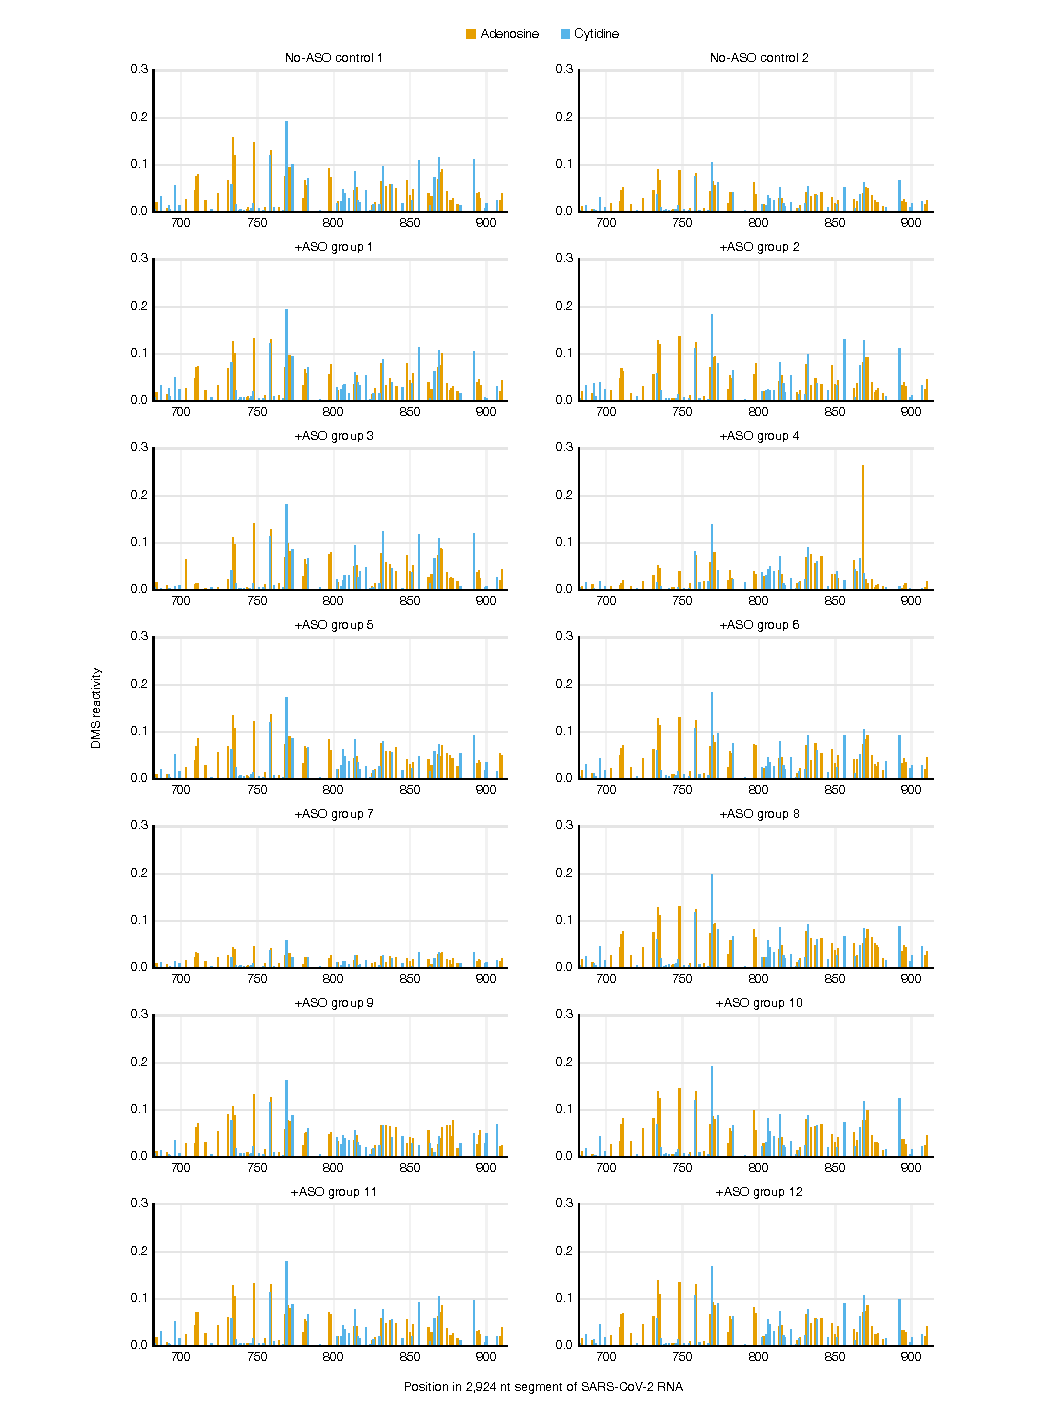
\includegraphics[width=\textwidth]{../SupplementaryFigures/sars2-tile-fse.pdf}
	\caption{\textbf{Mutational profiles of the FSE section upon adding each group of ASOs to the 2,924 nt segment of SARS-CoV-2 genomic RNA.} Positions are colored based on the RNA sequence.}
	\label{sars2-tile-fse}
\end{suppfigure}


\begin{suppfigure}[H]
	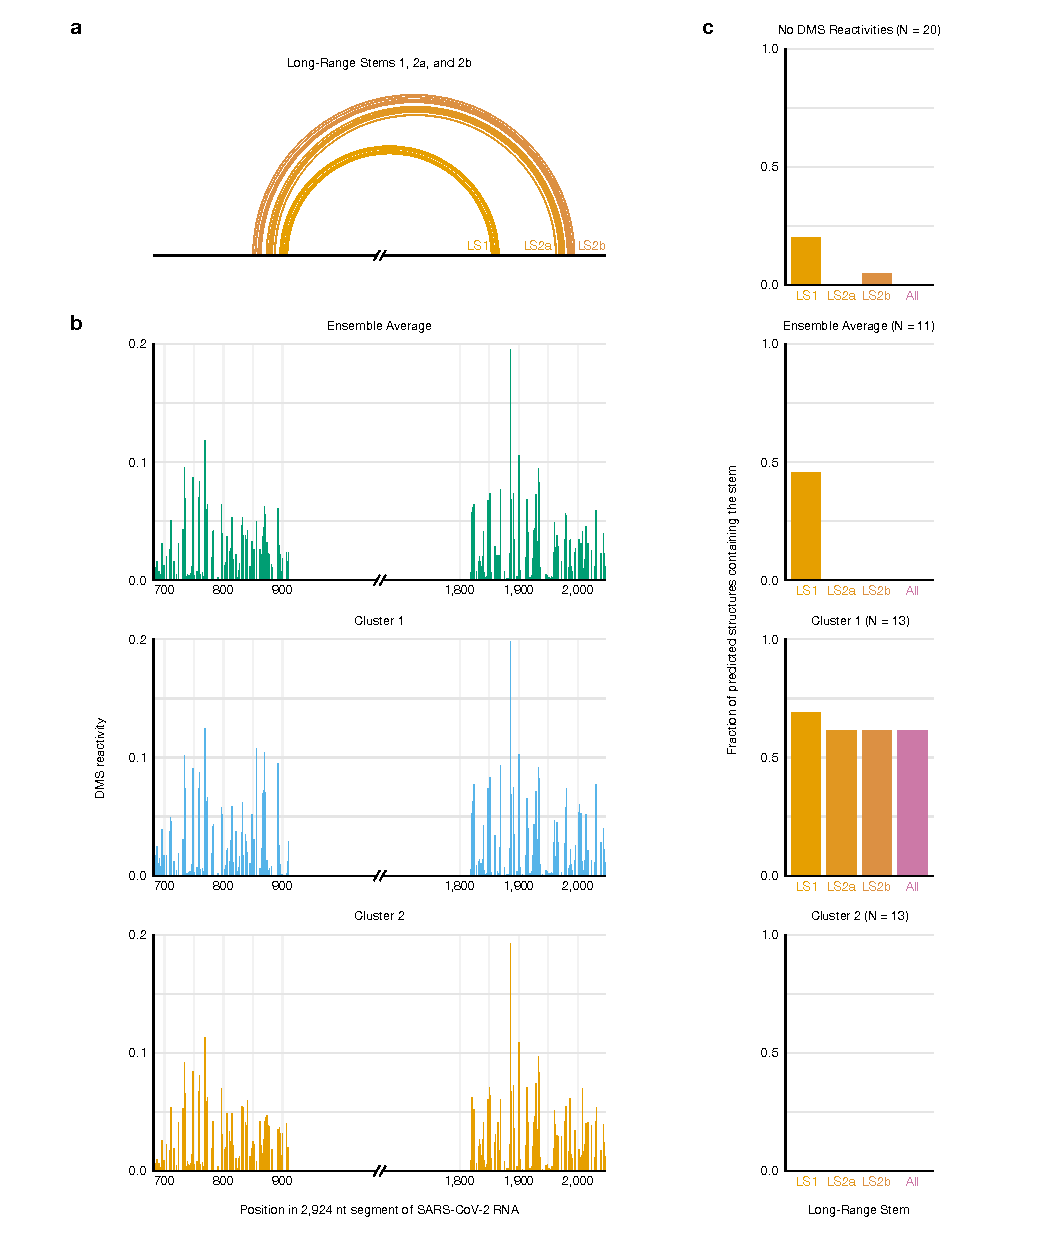
\includegraphics[width=\textwidth]{../SupplementaryFigures/sars2-clusters-fold.pdf}
	\caption{\textbf{Improved prediction of long-range stems in SARS-CoV-2 using clustered DMS reactivities.} \textbf{(a)} Model of the two inner stems of the FSE-arch, denoted long stems (LS) 1, 2a, and 2b. \textbf{(b)} Mutational profiles of the ensemble average and of clusters 1 and 2 on both sides of the FSE-arch. \textbf{(c)} For each mutational profile (as well as a purely thermodynamic prediction with no DMS reactivities), the fraction of predicted structures in which each long stem was predicted perfectly (i.e. all base pairs were present). The numbers of predicted structures (N) are indicated.}
	\label{sars2-clusters-fold}
\end{suppfigure}


\begin{suppfigure}[H]
	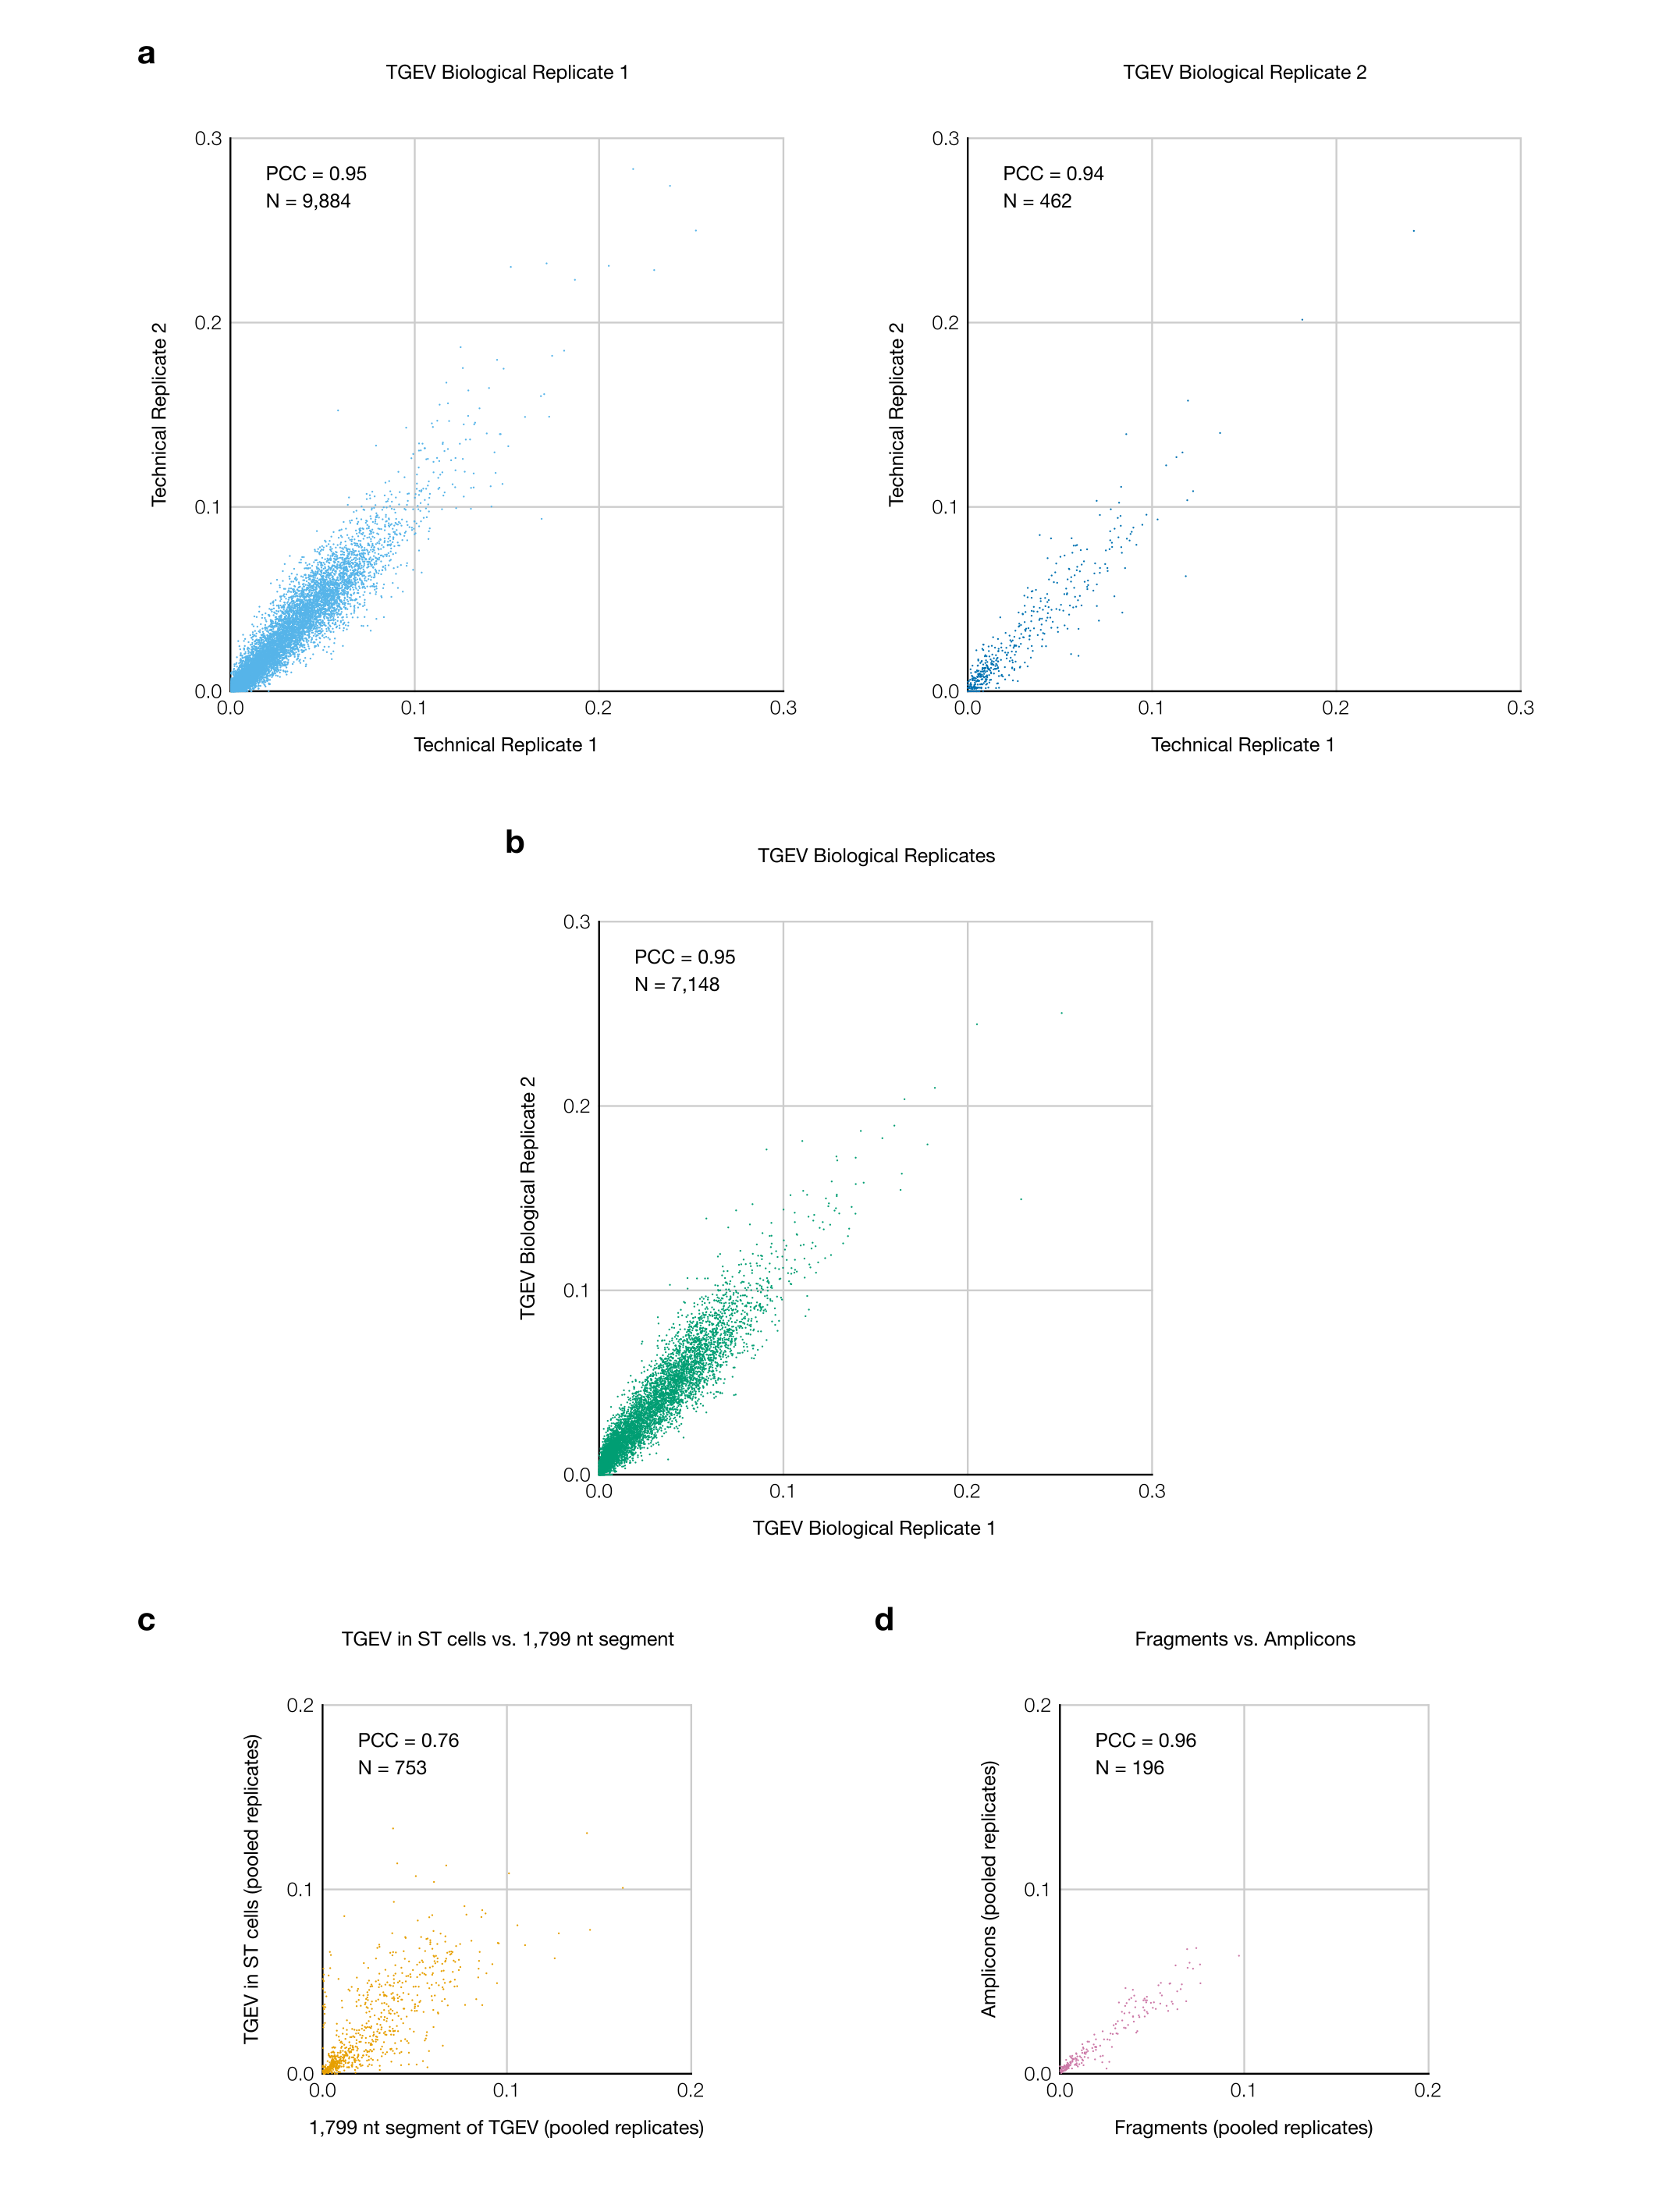
\includegraphics[width=\textwidth]{../SupplementaryFigures/tgev_reps.pdf}
	\caption{\textbf{Replicates of TGEV in ST cells and comparison to the 1,799 nt segment.} \textbf{(a)} Scatter plots comparing the DMS reactivities of the two technical replicates for each biological replicate of TGEV in ST cells. Each point represents one base in the sequence. The number of points (N) and Pearson correlation coefficient (PCC) are indicated for each plot. \textbf{(b)} Scatter plot comparing the DMS reactivities of the two biological replicates (each biological replicate comprises the reads for both of its technical replicates pooled together). \textbf{(c)} Scatter plot comparing the DMS reactivities of TGEV in ST cells (the reads for both biological replicates pooled together) and for the 1,799 nt segment \textit{in vitro}.}
	\label{tgev_reps}
\end{suppfigure}


\begin{suppfigure}[H]
	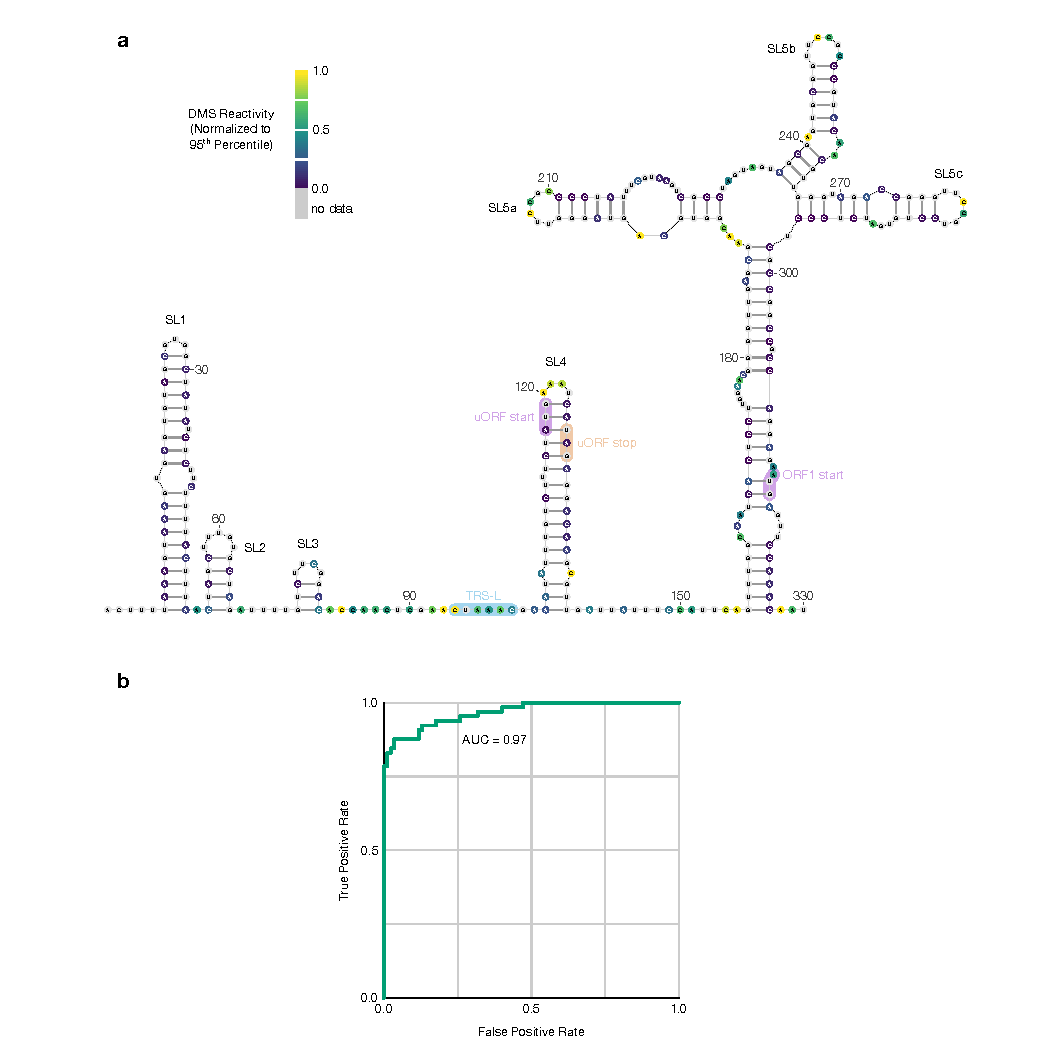
\includegraphics[width=\textwidth]{../SupplementaryFigures/tgev_5utr.pdf}
	\caption{\textbf{Secondary structure of the 5' UTR of TGEV.} \textbf{(a)} Model of the secondary structure of the first 520 nt of the TGEV genome, based on DMS reactivities in infected ST cells normalized to the 95\textsuperscript{th} percentile. Bases are colored by DMS reactivity. The model includes the highly conserved stem loops SL1, SL2, SL4, SL5a, SL5b, and SL5c, as well as the more variable stem loops SL3, SL6, SL7, and SL8~\cite{Yang2015a}. The leader transcription regulatory sequence (TRS-L)~\cite{Alonso2002}, upstream open reading frame (uORF)~\cite{Nakagawa2016}, and start codon of ORF1 are also labeled. The model was drawn using VARNA~\cite{Darty2009}. \textbf{(b)} Receiver operating characteristic curve showing agreement between the DMS reactivities and the secondary structure model; the area under the curve (AUC) is indicated.}
	\label{tgev_5utr}
\end{suppfigure}


\end{document}
